\documentclass[10pt,english,aspectratio=169]{beamer}
% Use notes or hide notes or show only notes or handout


\usetheme{default}

\usepackage{xstring}
\usepackage{pgfpages}
%\makeatletter
%\IfSubStr{\@classoptionslist}{handout}
%  {\pgfpagesuselayout{2 on 1}[letterpaper,border shrink=5mm]}
%  {}
%\makeatother

\usepackage{amsmath,amssymb,amsthm}
\usepackage{stmaryrd}
\usepackage{enumerate}
\usepackage{stfloats}
\usepackage{bbm}
\usepackage{pdfpages}
\usepackage{framed}
\usepackage{tabularx}
\usepackage{scalerel}

\usepackage[most]{tcolorbox}
\tcbset{highlight math style={enhanced,
  colframe=white,colback=yellow!15,arc=8pt,boxrule=1pt,
  }}
  
\usepackage{tikz,pgf,pgfplots}
\usepackage{algorithm,algorithmic}
\usepgflibrary{shapes}
\usetikzlibrary{%
  arrows,%
  arrows.meta,
  backgrounds,
  shapes.misc,% wg. rounded rectangle
  shapes.arrows,%
  shapes,%
  calc,%
  chains,%
  matrix,%
  positioning,% wg. " of "
  scopes,%
  decorations.pathmorphing,% /pgf/decoration/random steps | erste Graphik
  shadows,%
  backgrounds,%
  fit,%
  petri,%
  quotes
}

\tikzset{background rectangle/.style={
    fill=white,
  },
  use background/.style={    
    show background rectangle
  }
}

\setbeamersize{text margin left=10mm,text margin right=35mm}

\pgfplotsset{compat=1.12}

%\usetheme{Frankfurt}
%\usecolortheme{ldpc}
\useinnertheme{rounded}
\usecolortheme{whale}
\usecolortheme{orchid}

\newcommand{\ul}[1]{\underline{#1}}
\renewcommand{\Pr}{\mathbb{P}}

%% Setup slides and notes
\makeatletter
\IfSubStr{\@classoptionslist}{notes} { \IfSubStr{\@classoptionslist}{hide} {}{\IfSubStr{\@classoptionslist}{only} {}{\setbeameroption{show notes on second screen=right}}} }{}
\makeatother
%\setbeamertemplate{note page}{\pagecolor{yellow!5}\vfill\insertnote\vfill}

\newcommand{\getpdfpages}[2]{\begingroup
  \setbeamercolor{background canvas}{bg=}
  \addtocounter{framenumber}{1}
  \includepdf[pages={#1},%
  pagecommand={%
    \expandafter\def\expandafter\insertshorttitle\expandafter{%
      \insertshorttitle\hfill\insertframenumber\,/\,\inserttotalframenumber}}%
  ]{#2}
  \endgroup}

\newcommand{\backupbegin}{
   \newcounter{finalframe}
   \setcounter{finalframe}{\value{framenumber}}
}
\newcommand{\backupend}{
   \setcounter{framenumber}{\value{finalframe}}
}

 \setbeamercolor{bibliography entry author}{fg=black}
 \setbeamercolor{bibliography entry title}{fg=black}
 \setbeamercolor{bibliography entry location}{fg=black}
 \setbeamercolor{bibliography entry note}{fg=black}
 
 \setbeamerfont{bibliography item}{size=\footnotesize}
 \setbeamerfont{bibliography entry author}{size=\footnotesize}
 \setbeamerfont{bibliography entry title}{size=\footnotesize}
 \setbeamerfont{bibliography entry location}{size=\footnotesize}
 \setbeamerfont{bibliography entry note}{size=\footnotesize}
 \setbeamertemplate{bibliography item}{\insertbiblabel}
 
\newlength\tikzwidth
\newlength\tikzheight


\newcommand{\mc}[1]{\mathcal{#1}}
\newcommand{\mbb}[1]{\mathbb{#1}}
%\newcommand{\expt}{\mbb{E}}
%\newcommand{\dd}{\mathrm{d}}
%\usepackage{fixltx2e}

\newcommand{\Interior}[1]{\ensuremath{{#1}^{\circ}}}
\newcommand{\Closure}[1]{\ensuremath{\overline{#1}}}
\newcommand{\Complement}[1]{\ensuremath{{#1}^{c}}}

\newcommand{\Expect}{\ensuremath{\mathrm{E}}}
\newcommand{\vecnot}{\underline}
\newcommand{\RealNumbers}{\mathbb{R}}
\newcommand{\RationalNumbers}{\mathbb{Q}}
\newcommand{\ComplexNumbers}{\mathbb{C}}
\newcommand{\Real}{\mathrm{Re}}
\newcommand{\Span}{\mathrm{span}}
\newcommand{\Rank}{\mathrm{rank}}
\newcommand{\Nullity}{\mathrm{nullity}}
\newcommand{\Trace}{\mathrm{tr}}
\newcommand{\Diag}{\mathrm{diag}}
\DeclareMathOperator*{\esssup}{ess\,sup}
\newcommand{\dd}{\mathrm{d}}



\def\checkmark{\tikz\fill[scale=0.4](0,.35) -- (.25,0) -- (1,.7) -- (.25,.15) -- cycle;}
\def\greencheck{{\color{green}\checkmark}}
\def\scalecheck{\resizebox{\widthof{\checkmark}*\ratio{\widthof{x}}{\widthof{\normalsize x}}}{!}{\checkmark}}
\def\xmark{\tikz [x=1.4ex,y=1.4ex,line width=.2ex, red] \draw (0,0) -- (1,1) (0,1) -- (1,0);}
\def\redx{{\color{red}\xmark}}

\renewcommand{\footnotesep}{-2pt}


\begin{document}

\title{ECE 586: Vector Space Methods \\ Lecture 17: Best Approximation}
\author{Henry D. Pfister \\ Duke University}
\date{}
%\date{August 20th, 2020}
%\maketitle

\setbeamertemplate{navigation symbols}{}

\begin{frame}[plain]
	\titlepage
	
	\note{
		\vspace{8mm}
		\begin{enumerate}
			\setlength\itemsep{3mm}
			\color{red}
			\item Welcome to the 11th video lecture for ECE 586, Vector Space Methods. \\[2mm]
			Today, we'll finish our discussion of subspaces and bases and then move on to linear transforms.
		\end{enumerate}
	}
\end{frame}

\addtocounter{framenumber}{-1}
\setbeamertemplate{navigation symbols}{\textcolor{blue}{\footnotesize \insertframenumber ~/ \inserttotalframenumber}}

\begin{frame}{4.1: Best Approximation}

Let $W$ be a subspace of a Banach space $V$ and, for any $\vecnot{v} \in V$, consider finding a vector $\vecnot{w} \in W$ such that $\left\| \vecnot{v} - \vecnot{w} \right\|$ is as small as possible.
\begin{definition}<1->
The vector $\vecnot{w} \in W$ is a \textcolor{blue}{best approximation} of $\vecnot{v} \in V$ by vectors in $W$ if \vspace{-1.5mm}
\begin{equation*}
\left\| \vecnot{v} - \vecnot{w} \right\| \leq \left\| \vecnot{v} - \vecnot{w}' \right\|, \vspace{-2.5mm}
\end{equation*}
for all $\vecnot{w}' \in W$.
\end{definition}

\begin{example}<2->
If $W$ is spanned by the vectors $\vecnot{w}_1, \ldots, \vecnot{w}_n \in V$, then we can write \vspace{-1.5mm}
\begin{equation*}
\vecnot{v} = \vecnot{w} + \vecnot{e} = s_1 \vecnot{w}_1 + \cdots + s_n \vecnot{w}_n + \vecnot{e}, \vspace{-1.5mm}
\end{equation*}
where $\vecnot{e} = \vecnot{v}-\vecnot{w}$ is the approximation error.
\end{example}
\end{frame}

\begin{frame}{Vector Projection Revisited}

Let $\vecnot{u},\vecnot{v}$ be vectors in an inner-product space $V$ with inner product $\tinner{ \cdot }{ \cdot }$.

\vspace{-1mm}

\begin{lemma}<1->
If $\tinner{ \vecnot{w} }{ \vecnot{v} } = 0$, then $\| \vecnot{w} \!+\! \vecnot{v} \|^2 = \| \vecnot{w} \|^2 \!+\! 2\, \text{Re} \{ \tinner{ \vecnot{w} }{ \vecnot{v} }  \} \!+\! \| \vecnot{v} \|^2 = \| \vecnot{w} \|^2 \!+\! \| \vecnot{v} \|^2$.
\end{lemma}

\vspace{-1mm}

\begin{definition}[Vector Projection]<1->
The \textcolor{blue}{projection} of $\vecnot{w}$ onto $\vecnot{v}$ is defined to be \\[-4mm]
\begin{tabular}{>{\centering}m{2.5in} m{2.5in}}
$ \vecnot{u} = \displaystyle\frac{\inner{ \vecnot{w} }{ \vecnot{v} }}{\|\vecnot{v}\|^2} \vecnot{v} $ &
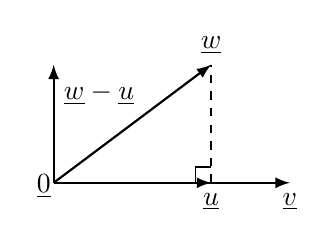
\begin{tikzpicture}[scale=0.5]
  \coordinate (v1) at (0,0);
  \coordinate (v2) at (4,3);
  \coordinate (v3) at (6,0);
  \coordinate (v4) at (4,0);
  \coordinate (v5) at (0,3);
  \path[draw] (3.6,0) -- (3.6,0.4) -- (4,0.4);
  \node (v0) at (-0.25,-0.1) {$\vecnot{0}$};
  \draw[-latex,thick] (v1) -- node[at end,above] {$\vecnot{w}$} (v2);
  \draw[-latex,thick] (v1) -- node[at end,below] {$\vecnot{v}$} (v3);
  \draw[-latex,thick] (v1) -- node[at end, below] {$\vecnot{u}$} (v4);
  \draw[thick,dashed] (v4) --  (v2);
  \draw[-latex,thick] (v1) -- node[right,near end] {$\vecnot{w}-\vecnot{u}$} (v5);
\end{tikzpicture}
\end{tabular}
\vspace{-2.5mm}
\end{definition}

\vspace{-1mm}


\begin{lemma}<2->
Let $\vecnot{u}$ be the projection of $\vecnot{w}$ onto $\vecnot{v}$.
If $\tinner{ \vecnot{w} }{ \vecnot{v} } \neq 0$, then $\| \vecnot{w} - \vecnot{u} \| < \| \vecnot{w} \|$.
\end{lemma}

\vspace{-1mm}
\begin{proof}<3->
$\tinner{ \vecnot{w} - \vecnot{u} }{ \vecnot{u} } = 0$ implies $\| \vecnot{w} \|^2 = \| (\vecnot{w}-\vecnot{u}) + \vecnot{u} \|^2 = \| \vecnot{w} -\vecnot{u} \|^2 + \| \vecnot{u} \|^2$.
\end{proof}

\end{frame}

\begin{frame}{4.1: Orthogonal Projection}

In an arbitrary Banach space, finding a best approximation can be hard.
\vspace{0.5mm}

For the induced norm of a Hilbert space, \textcolor{blue}{orthogonal projection} simplifies this!

\begin{theorem}[Projection] Suppose $W$ is a subspace of a Hilbert space $V$ and $\vecnot{v} \in V$.
Then,
\begin{enumerate}
\item The vector $\vecnot{w} \in W$ is a best approximation of $\vecnot{v} \in V$ by vectors in $W$ if and only if $\vecnot{v} - \vecnot{w}$ is orthogonal to every vector in $W$.
\item If a best approximation of $\vecnot{v} \in V$ by vectors in $W$ exists, it is unique.
\item If $W$ is a closed subspace with a countable orthogonal basis $\vecnot{w}_1, \vecnot{w}_2, \ldots$, then the best approximation of $\vecnot{v}$ by vectors in $W$ is \vspace{-1.5mm}
\begin{equation*}
\vecnot{w} = \sum_{i=1}^{\dim (W)} \frac{ \inner{ \vecnot{v} }{ \vecnot{w}_i } }{ \left\| \vecnot{w}_i \right\|^2 } \vecnot{w}_i . \vspace{-1mm}
\end{equation*}
Note: the implied linear mapping $T\colon V \to W$ defined by $T(\vecnot{v}) = \vecnot{w}$ is called the \textcolor{blue}{orthogonal projection} of $V$ onto $W$.
\end{enumerate}
\end{theorem}

Proof in live session.

\end{frame}


\begin{frame}{Orthogonal Projection Example}

\begin{example}<1->
For the standard inner product space $V = \mathbb{R}^3$, let $W$ be the subspace spanned by\vspace{-4mm}
\begin{align*}
\vecnot{v}_1 &= (2,2,1), \\
\vecnot{v}_2 &= (3,6,0).
\end{align*}
Then, the Gram-Schmidt process generates the orthogonal basis
 \vspace{-2mm}
\begin{align*}
\vecnot{w}_1 &= (2,2,1), \\
\vecnot{w}_2 &= (-1,2,-2)
\end{align*}
and the orthogonal projection of $\vecnot{v} \in V$ onto $W$ is defined by \vspace{-2mm}
\begin{align*}
T \vecnot{v} &= \sum_{i=1}^2 \frac{ \inner{ \vecnot{v} }{ \vecnot{w}_i } }{ \left\| \vecnot{w}_i \right\|^2 } \vecnot{w}_i \\ &= \frac{1}{9} \inner{ \vecnot{v} }{ (2,2,1) } (2,2,1) + \frac{1}{9} \inner{ \vecnot{v} }{ (-1,2,-2) } (-1,2,-2).
\end{align*}
\vspace*{-3.5mm}
\end{example}

\end{frame}


\newcommand*{\vertbar}{\rule[-1ex]{0.5pt}{2.5ex}}

\begin{frame}{4.1.1: Orthogonal Projection onto an Orthonormal Set}

Let $V = \ComplexNumbers^n$ be the standard $n$-dimensional complex Hilbert space and $U \in \ComplexNumbers^{n\times m}$ be a matrix with orthonormal columns $\vecnot{u}_1,\ldots,\vecnot{u}_m$:

\[ U = \begin{bmatrix} \vertbar & \vertbar & & \vertbar \\ \vecnot{u}_1 & \vecnot{u}_2 & \cdots & \vecnot{u}_m \\ \vertbar & \vertbar & & \vertbar \end{bmatrix} \]

\vspace{4mm}

Then, the best approximation of $\vecnot{v}\in V$ by vectors in $\mathcal{R}(U)$, given by
\begin{equation*}
\vecnot{w} = \sum_{i=1}^m \frac{ \inner{ \vecnot{v} }{ \vecnot{u}_i } }{ \left\| \vecnot{u}_i \right\|^2 } \vecnot{u}_i,
\end{equation*}
can also be written as
\[ {\color{blue}\vecnot{w} = U U^H \vecnot{v}} = \sum_{i=1}^m \vecnot{u}_i (\vecnot{u}_i^H \vecnot{v}). \]

\end{frame}




\begin{frame}{4.1.1: What is a Projection? (1)}

\begin{definition}
A function $F \colon X \rightarrow Y$ with $Y \subseteq X$ is \textcolor{blue}{idempotent} if $F(F(x))=F(x)$.  When $F$ is a linear transformation, this reduces to $F^2 = F \cdot F = F$.
\end{definition}

\begin{definition}
Let $V$ be a vector space and $T \colon V \rightarrow V$ be a linear transformation.
If $T$ is idempotent, then $T$ is called a \textcolor{blue}{projection} because $T\vecnot{v} = \vecnot{v}$ if $\vecnot{v} \in \mathcal{R}(T)$.
\end{definition}

\begin{example}
The idempotent matrix $A$ is a projection onto the first two coordinates. \vspace{-2mm}
\begin{equation*}
A = \begin{bmatrix}
1 & 0 & 1 \\
0 & 1 & 1 \\
0 & 0 & 0
\end{bmatrix}
\end{equation*}
\end{example}

\end{frame}

\begin{frame}{4.1.1:  What is a Projection? (2)}

\begin{theorem}
Let $V$ be a vector space and $T \colon V \rightarrow V$ be a (linear) projection operator.
Then, the range $\mathcal{R}(T)$ and the $\mathcal{N}(T)$ are disjoint subspaces of $V$.
\end{theorem}

\begin{proof}
For a non-zero $\vecnot{v} \in \mathcal{R}(T)$, there is a non-zero $\vecnot{w} \in V$ such that $\vecnot{v} = T\vecnot{w}$.  Thus, $T\vecnot{v} = T^2  \vecnot{w} = T \vecnot{w} = \vecnot{v} \neq \vecnot{0}$.  But, if $\vecnot{v} \in \mathcal{N}(T)$ was also true, then one would get the contradiction $T\vecnot{v} = \vecnot{0}$.
\end{proof}

\begin{example}<2->
Consider the linear transform $T \colon V \rightarrow V$ defined by $T = I - P$, where $P$ is a projection.
It is easy to verify that $T$ is a projection operator because \vspace{-2mm}
\[ T^2 = (I-P)(I-P) = I - P- P + P^2 = I-P = T .\]
In fact, $T$ is a projection onto $\mathcal{R}(T) = \mathcal{N}(P)$ because $P \vecnot{v} = \vecnot{0}$ (i.e., $\vecnot{v} \in \mathcal{N}(P)$) if and only if  $(I-P)\vecnot{v} = \vecnot{v}$ (i.e., $\vecnot{v} \in \mathcal{R}(T)$).
\end{example}

\end{frame}

\begin{frame}{4.1.1: Orthogonal Projection Operators}

\vspace{-1mm}

\begin{definition}<1->
Let $V$ be an inner-product space and $P \colon V \rightarrow V$ be a (linear) projection operator.
If $\smash{\mathcal{R}(P) \bot \mathcal{N}(P)}$, then $P$ is called an \textcolor{blue}{orthogonal projection}.
\end{definition}

\vspace{-1mm}

\begin{example}<1->
Let $V$ be an inner-product space $P \colon V \rightarrow V$ be an orthogonal projection.
Then, $\vecnot{v} = P \vecnot{v} + (I-P) \vecnot{v}$ gives an orthogonal decomposition of $\vecnot{v}$ because $P \vecnot{v} \in \mathcal{R}(P)$, $(I-P) \vecnot{v} \in \mathcal{N}(P)$, and $\mathcal{R}(P) \bot \mathcal{N}(P)$.
\end{example}

\vspace{-1mm}

\begin{theorem}<2->
For $V=F^n$ with standard inner product, $P$ is an orthogonal projection matrix if it is idempotent and Hermitian (i.e. $P^2=P$ and $P^H = P$).
\end{theorem}

\vspace{-1mm}

\begin{proof}<3->
Since $\mathcal{R}(P) = \{ P\vecnot{u} | \vecnot{u}\in V \}$ and $\mathcal{N}(P) = \{ \vecnot{v}\in V | P\vecnot{v}=\vecnot{0} \}$, the general condition is $\tinner{ P\vecnot{u} }{ (I-P)\vecnot{v} } =0$ for all $\vecnot{u},\vecnot{v}\in V$.
Simplifying this gives \vspace{-2mm}
\[ \vecnot{v}^H (I-P)^H P \vecnot{u} = \vecnot{v}^H (P - P^H P) \vecnot{u} = \vecnot{v}^H (P - P^2) \vecnot{u} = 0.  \qedhere\]
\end{proof}

\end{frame}


\begin{frame} \frametitle{Next Steps}

\begin{itemize}
\setlength\itemsep{5mm}
\item To continue studying after this video -- \vspace{2mm}

\begin{itemize}
 \setlength\itemsep{3mm}
 \item Try the required reading: Course Notes EF 4.1 - 4.1.1
 \item Or the recommended reading: LADR 6C
 \item Also, look at the problems in Assignment 7
\end{itemize}
\end{itemize}

\note{
	\vspace{8mm}
	\begin{enumerate}
		\setlength\itemsep{3mm}
		\color{red}
		\item Here are some options to continue learning this material. (read) \\ [2mm]  That's it for today.  So, I'll see you next time.
	\end{enumerate}
}

\end{frame}


\end{document}




